\documentclass{article}

\usepackage{tikz}
\usepackage{cancel}%for strikethrough
\usetikzlibrary{positioning}

\begin{document}


\begin{figure}
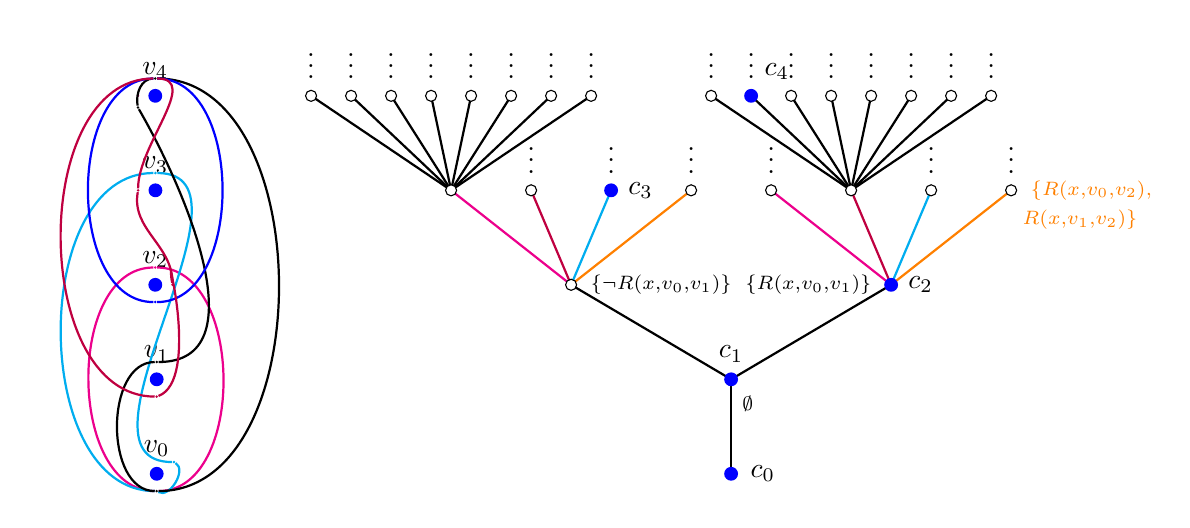
\begin{tikzpicture}[grow'=up,scale=.8]
\tikzstyle{level 1}=[sibling distance=3.3in]
\tikzstyle{level 2}=[sibling distance=2in]
\tikzstyle{level 3}=[sibling distance=.5in]
\tikzstyle{level 4}=[sibling distance=0.25in]
\tikzstyle{level 5}=[sibling distance=0.125in]
\node [label=0:$c_0$] {} coordinate (t9)
child{ coordinate (t0) edge from parent[color=black,thick]
child{ coordinate (t00) edge from parent[color=black,thick]
child{ coordinate (t000) edge from parent[color=magenta,thick]
child{coordinate (t0000) edge from parent[color=black,thick]}
child{coordinate (t0001) edge from parent[color=black,thick]}
child{coordinate (t0002) edge from parent[color=black,thick]}
child{coordinate (t0003) edge from parent[color=black,thick]}
child{coordinate (t0004) edge from parent[color=black,thick]}
child{coordinate (t0005) edge from parent[color=black,thick]}
child{coordinate (t0006) edge from parent[color=black,thick]}
child{coordinate (t0007) edge from parent[color=black,thick]}
}%endparen for t000
child{coordinate (t001) edge from parent[color=purple,thick]}
child{coordinate (t002) edge from parent[color=cyan,thick]}
child{coordinate (t003) edge from parent[color=orange,thick]}
}%endparen t00
child{ coordinate (t01) edge from parent[color=black,thick]
child{ coordinate (t010) edge from parent[color=magenta,thick]}
child{ coordinate (t011) edge from parent[color=purple,thick]
child{ coordinate (t0110) edge from parent[color=black,thick]}
child{ coordinate (t0111) edge from parent[color=black,thick]}
child{ coordinate (t0112) edge from parent[color=black,thick]}
child{ coordinate (t0113) edge from parent[color=black,thick]}
child{ coordinate (t0114) edge from parent[color=black,thick]}
child{ coordinate (t0115) edge from parent[color=black,thick]}
child{ coordinate (t0116) edge from parent[color=black,thick]}
child{ coordinate (t0117) edge from parent[color=black,thick]}
}
child{ coordinate (t012) edge from parent[color=cyan,thick]}
child{ coordinate (t013) edge from parent[color=orange,thick]}
}%endparen for t01
}%endparen for t0
;
%line spaces make a difference!!!


\node[circle, fill=blue,inner sep=0pt, minimum size=5pt] at (t9) {};
\node[circle, fill=blue,inner sep=0pt, minimum size=5pt,label=90:$c_1$,label=280:$\scriptstyle{\emptyset}$] at (t0) {};
\node[circle, fill=blue,inner sep=0pt, minimum size=5pt,label=0:$c_2$] at (t01) {};
\node[circle, fill=blue,inner sep=0pt, minimum size=5pt,label=0:$c_3$] at (t002) {};
\node[circle, fill=blue,inner sep=0pt, minimum size=5pt,label=60:$c_4$] at (t0111) {};
\node[label=0:$\scriptstyle{\{\neg R(x,v_0,v_1)\}}$] at (t00) {};
\node[label=180:$\scriptstyle{\{R(x,v_0,v_1)\}}$] at (t01) {};
\node[label=280:${\color{orange}\scriptstyle{R(x,v_1,v_2)\}}}$,label=0:${\color{orange}\scriptstyle{\{R(x,v_0,v_2),}}$] at (t013) {};

%open circles for additional nodes
\node[circle, fill=white,draw,inner sep=0pt, minimum size=4pt] at (t00) {};
\node[circle, fill=white,draw,inner sep=0pt, minimum size=4pt] at (t000) {};
\node[circle, fill=white,draw,inner sep=0pt, minimum size=4pt] at (t001) {};
\node[circle, fill=white,draw,inner sep=0pt, minimum size=4pt] at (t003) {};
\node[circle, fill=white,draw,inner sep=0pt, minimum size=4pt] at (t0000) {};
\node[circle, fill=white,draw,inner sep=0pt, minimum size=4pt] at (t0001) {};
\node[circle, fill=white,draw,inner sep=0pt, minimum size=4pt] at (t0002) {};
\node[circle, fill=white,draw,inner sep=0pt, minimum size=4pt] at (t0003) {};
\node[circle, fill=white,draw,inner sep=0pt, minimum size=4pt] at (t0004) {};
\node[circle, fill=white,draw,inner sep=0pt, minimum size=4pt] at (t0005) {};
\node[circle, fill=white,draw,inner sep=0pt, minimum size=4pt] at (t0006) {};
\node[circle, fill=white,draw,inner sep=0pt, minimum size=4pt] at (t0007) {};
\node[circle, fill=white,draw,inner sep=0pt, minimum size=4pt] at (t010) {};
\node[circle, fill=white,draw,inner sep=0pt, minimum size=4pt] at (t011) {};
\node[circle, fill=white,draw,inner sep=0pt, minimum size=4pt] at (t012) {};
\node[circle, fill=white,draw,inner sep=0pt, minimum size=4pt] at (t013) {};
\node[circle, fill=white,draw,inner sep=0pt, minimum size=4pt] at (t0110) {};
\node[circle, fill=white,draw,inner sep=0pt, minimum size=4pt] at (t0112) {};
\node[circle, fill=white,draw,inner sep=0pt, minimum size=4pt] at (t0113) {};
\node[circle, fill=white,draw,inner sep=0pt, minimum size=4pt] at (t0114) {};
\node[circle, fill=white,draw,inner sep=0pt, minimum size=4pt] at (t0115) {};
\node[circle, fill=white,draw,inner sep=0pt, minimum size=4pt] at (t0116) {};
\node[circle, fill=white,draw,inner sep=0pt, minimum size=4pt] at (t0117) {};

%making the collection of v nodes
\node[circle, fill=blue,inner sep=0pt, minimum size=5pt, label=$v_0$,left=7.2cm of t9] (v0) {};
\node[circle, fill=blue,inner sep=0pt, minimum size=5pt, label=$v_1$,left=7.2cm of t0] (v1) {};
\node[circle, fill=blue,inner sep=0pt, minimum size=5pt, label=$v_2$,left=9.25cm of t01] (v2) {};
\node[circle, fill=blue,inner sep=0pt, minimum size=5pt, label=$v_3$,left=3.66cm of t000] (v3) {};
\node[circle, fill=blue,inner sep=0pt, minimum size=5pt, label=$v_4$,left=7.98cm of t0112] (v4) {};

%vdots on the top nodes
\node[circle,inner sep=0pt, minimum size=5pt,label=90:$\vdots$] at (t0000) {};
\node[circle,inner sep=0pt, minimum size=5pt,label=90:$\vdots$] at (t0001) {};
\node[circle,inner sep=0pt, minimum size=5pt,label=90:$\vdots$] at (t0002) {};
\node[circle,inner sep=0pt, minimum size=5pt,label=90:$\vdots$] at (t0003) {};
\node[circle,inner sep=0pt, minimum size=5pt,label=90:$\vdots$] at (t0004) {};
\node[circle,inner sep=0pt, minimum size=5pt,label=90:$\vdots$] at (t0005) {};
\node[circle,inner sep=0pt, minimum size=5pt,label=90:$\vdots$] at (t0006) {};
\node[circle,inner sep=0pt, minimum size=5pt,label=90:$\vdots$] at (t0007) {};
\node[circle,inner sep=0pt, minimum size=5pt,label=90:$\vdots$] at (t001) {};
\node[circle,inner sep=0pt, minimum size=5pt,label=90:$\vdots$] at (t002) {};
\node[circle,inner sep=0pt, minimum size=5pt,label=90:$\vdots$] at (t003) {};
\node[circle,inner sep=0pt, minimum size=5pt,label=90:$\vdots$] at (t010) {};
\node[circle,inner sep=0pt, minimum size=5pt,label=90:$\vdots$] at (t012) {};
\node[circle,inner sep=0pt, minimum size=5pt,label=90:$\vdots$] at (t013) {};
\node[circle,inner sep=0pt, minimum size=5pt,label=90:$\vdots$] at (t0110) {};
\node[circle,inner sep=0pt, minimum size=5pt,label=90:$\vdots$] at (t0111) {};
\node[circle,inner sep=0pt, minimum size=5pt,label=90:$\vdots$] at (t0112) {};
{};
\node[circle,inner sep=0pt, minimum size=5pt,label=90:$\vdots$] at (t0113) {};
{};
\node[circle,inner sep=0pt, minimum size=5pt,label=90:$\vdots$] at (t0114) {};
{};
\node[circle,inner sep=0pt, minimum size=5pt,label=90:$\vdots$] at (t0115) {};
{};
\node[circle,inner sep=0pt, minimum size=5pt,label=90:$\vdots$] at (t0116) {};
{};
\node[circle,inner sep=0pt, minimum size=5pt,label=90:$\vdots$] at (t0117) {};

%making phantom nodes for the curves
\node[circle,fill=black,inner sep=0pt, minimum size=1pt,below=.1cm of v0] (u0) {};
\node[circle,fill=purple,inner sep=0pt, minimum size=1pt,below=.1cm of v1] (u1) {};
\node[circle,fill=magenta,inner sep=0pt, minimum size=1pt,above=.1cm of v2] (a2) {};
\node[circle,fill=black,inner sep=0pt, minimum size=1pt,above=.1cm of v1] (a1) {};
\node[circle,fill=blue,inner sep=0pt, minimum size=1pt,below=.1cm of v2] (u2) {};
\node[circle,fill=purple,inner sep=0pt, minimum size=1pt,right=.1cm of v2] (r2) {};
\node[circle,fill=cyan,inner sep=0pt, minimum size=1pt,above=.1cm of v3] (a3) {};
\node[circle,fill=purple,inner sep=0pt, minimum size=1pt,left=.1cm of v3] (l3) {};
\node[circle,fill=white,inner sep=0pt, minimum size=1pt,left=.1cm of v1] (l1) {};
\node[circle,fill=white,inner sep=0pt, minimum size=1pt,right=.1cm of v0] (r0) {};
\node[circle,fill=cyan,inner sep=0pt, minimum size=1pt,above=.1cm of r0] (ar0) {};
\node[circle,fill=black,inner sep=0pt, minimum size=1pt,above=.1cm of v4] (a4) {};
\node[circle,fill=magenta,inner sep=0pt, minimum size=1pt,left=.1cm of v4] (l4) {};
\node[circle,fill=black,inner sep=0pt, minimum size=1pt,below=.1cm of l4] (ul4) {};

%arcs
\draw[magenta,thick] (u0) to [out=180,in=180] (a2);
\draw[magenta,thick] (u0) to [in=0,out=0] (a2);

\draw[cyan,thick] (u0) to [in=180,out=180] (a3);
\draw[cyan,thick] (a3) to [in=180,out=0] (ar0);
\draw[cyan,thick] (ar0) to [in=-30,out=-30] (u0);

\draw[black,thick] (u0) to [in=180,out=180] (a1);
\draw[black,thick] (a4) to [in=0,out=0] (u0);
\draw[black,thick] (a1) to [in=300,out=0] (ul4);
\draw[black,thick] (ul4) to [in=180,out=100] (a4);

\draw[blue,thick] (u2) to [out=180,in=180] (a4);
\draw[blue,thick] (a4) to [in=0,out=0] (u2);

\draw[purple,thick] (a4) to [in=180,out=180] (u1);
\draw[purple,thick] (u1) to [in=100,out=20] (r2);
\draw[purple,thick] (r2) to [in=260,out=90] (l3);
\draw[purple,thick] (l3) to [in=0,out=90] (a4);
\end{tikzpicture}
\end{figure}



\end{document}